\chapter{Referencial Teórico}
\label{cap:referencial_teorico}
\section{Virtualização}
No contexto da computação, frequetemente uma alteração tecnológica torna alguma idéia obsoleta e ela desaparece rapidamente. Entretanto, outra mudança tecnológica poderia reavivá-la \cite{tanembaum}. Este é o caso da virtualização, dado que sua utilização teve oscilações ao longo do tempo. A principal motivação para virtualização nos começo dos anos 70 era aumentar o nivel de compartilhamento e utilização dos caros recursos computacionais tais como \textit{mainframes}\cite{menasce}. Nos anos 80 com a queda dos custos de hardware as grandes corporações trocaram os grandes e despediosos \textit{mainframes} por coleções de computadores pessoais, tendo assim a virtualização caído em desuso.

 Seu ressurgimento só viria acontecer, nos anos 90 dentro de um contexto ao qual tinha-se o crescimento de novos paradigmas computacionais, tais como cliente-servidor  e sistemas \textit{peer-to-peer}, aos quais em suas estruturas eram constituídas basicamente de máquinas clientes conectadas à vários servidores.Esses novos ambientes trouxeram com eles diversos desafios e problemas incluindo confiabilidade, segurança, aumento no custo de administração e complexidade, espaço fisico e consumo de energia \cite{menasce}. Desse modo, o ressurgimento da virtualização vem promovendo a mitigação de tais problemas recorrentes nesses novos paradigmas computacionais ( alteração tecnológica).
 
\subsection{Conceituação}
Pode se definir que Virtualização é a técnica que permite particionar um único sistema computacional em vários outros denominados de máquinas virtuais. Cada máquina virtual oferece um ambiente completo muito similar a uma máquina física. Com isso, cada máquina virtual pode ter seu próprio sistema operacional, aplicativos e serviços de rede (Internet) \cite{carissimi}. A virtualização pode ser feita das seguintes formas:

\begin{itemize}
\item \textbf{Virtualização de servidores:} a mais comum e fácil de ser justificada. Diferente da época dos \textit{mainframes}, a virtualização agora é feita em servidores \textit{x86}.

\item \textbf{Virtualização de desktops:} trata da configuração dos desktops dos usuários finais em uma infraestrutura centalizada virtual. Isso signfica que as aplicações de desktop também passam a executar em um datacenter, sob a forma de máquinas virtuais.Esse é o conceito de \textit{Virtual Desktop Infrastructure(VDI)}, que permite a montagem dinâmica de desktops, oferecendo maior confiabilidade e otimização do uso de espaço em disco com a consollidação do armazenamento e flexibilidade na escolha do sistema peracional \cite{manoel}.

\item \textbf{Virtualização do armazenamento(\textit{storage})}: a ideia é introduzir um componente que permite às diversas unidade heterogêneas de armazenamento(discos físicos) serem vistas como um conjunto homogêneo de recursos \cite{manoel}.

\item \textbf{Virtualização das aplicações:} trata do conceito de execução do programa por completo, em um repositório central, permitindo a configuração centralizada do aplicativo, o que melhora seu gerenciamento, por permitir que seja feita em um único lugar \cite{manoel}. 

\item \textbf{Virtualização de redes: } Arquitetura que proporciona um ambiente de rede separado para cada grupo ou organização. Esses ambientes lógicos são criados sobre uma única infraestrutura compartilhada de rede \cite{manoel}.

\end{itemize}

Uma outra abordagem que pode ser utilizada para conceituar a virtualização é defini-la como uma camada de abstração entre o hardware e o software, que protege o acesso direto do software aos recursos físicos do hardware. A forma pela qual essa camada de abstração é implementada dá origem às máquinas virtuais de processo e aos monitores de máquinas virtuais também chamados de hipervisores \cite{manoel}.

\begin{figure}[!htb]
\centering
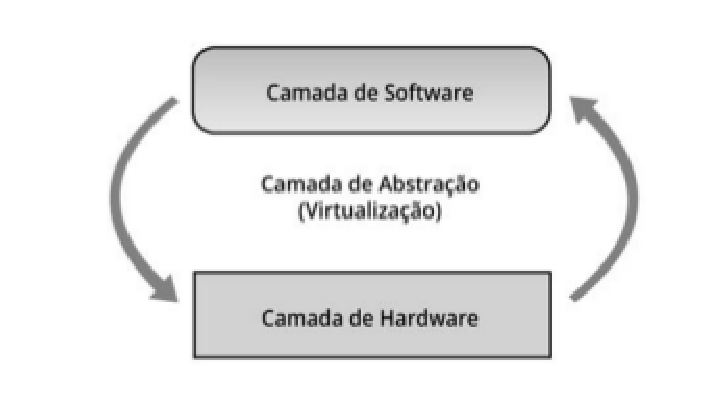
\includegraphics [keepaspectratio=true,scale=0.60]{figuras/virtualization_role.eps}
\caption{Responsabilidade da virtualização}
\cite{manoel}.
\label{virtualization_role}
\end{figure}

\subsection{Monitor de Máquinas Virtuais}



\section{Computação em Nuvem}